% !TeX spellcheck = en_GB
\documentclass[titlepage]{article}
\usepackage[margin=1.2in]{geometry}
\usepackage{amsfonts,amsthm,bm, amssymb} 
\usepackage[]{amsmath}
\usepackage{tikz}
\usepackage{listings}
\lstset{language = R, 
	basicstyle = \ttfamily, 
	commentstyle=\color{blue}\ttfamily,
	keywordstyle=\ttfamily
}
%\renewcommand{\ttdefault}{pcr}
\usepackage{graphicx}
\graphicspath{{images/}}
\usepackage{courier}
\usepackage{array}
\usepackage{enumitem}
\usepackage{booktabs}
\usepackage{float}
\usepackage[export]{adjustbox}

\title{ACTL3162 General Insurance Techniques Assignment}
\author{Johnny Wong, z5016960}

\begin{document}
	\maketitle
	\tableofcontents
	\newpage
	\section{Task 1}
	\subsection{Summary}
	The Maximum Likelihood Estimator (MLE) was found for 3 distributions: Pareto, Log-normal, and Gamma. It was found that the Log Normal distribution fit this data the best.\\
	
	The following table summarises the estimated parameters and their associated Aikaike Information Criteria (AIC). The AIC captures information concerning the  of goodness of fit of the data to the model and the need to build a model with many variables. Since we're fitting all models to the same data, and all three models have 2 parameters to fit, the AIC, BIC, and likelihood measures are all essentially equivalent.
	
	\begin{center}
		\begin{tabular}{ |c|c|c|c|} 
			\hline
			Distribution & Parameter 1 & Parameter 2 & AIC \\ \hline
			Pareto & $ \alpha = 51.18 $ & $\lambda = 200,000$ & 22,033.600\\ 
			Log-Normal & $\mu = 8.432$ & $\sigma = 0.396$ & 21,146.657 \\ 
			Gamma & $\alpha = 6.555$ & $\beta = 0.001$ & 21,156.529 \\ 
			\hline
		\end{tabular}
	\end{center}

	Furthermore, the empirical and theoretical distributions are plotted. 
	Through visual means, it is obvious that the Pareto distribution is not an appropriate fit for the data. 
	Additionally, the Log Normal distribution seems to deviate less from the empirical data than the Gamma distribution, suggesting a better fit to the Log Normal distribution.\\
	P-P and Q-Q plots were created and revealed that the Log Normal distribution tends to overestimate the tail, whereas the Gamma distribution underestimates it. In the context of modelling insurance claims, it is better to have a model that overestimates claim size rather than one that underestimates. This leads to higher reserves and a lower probability of ruin.
	\\
	Hypothesis tests were also conducted, concluding that the data is not Pareto distributed, but could be Log Normal or Gamma. The hypothesis tests favoured the Log Normal distribution over the Gamma.\\
	Through the combination of both statistical and visual analysis, it is concluded that the Log-Normal distribution is the most appropriate distribution to fit to the data, followed closely by the Gamma distribution.
	\subsection{General procedure}
	The MLE is calculated by first finding the likelihood function. This is simply the product of the probability density function (PDF) evaluated at each data point. Furthermore, each the contribution of the PDF from each datapoint is adjusted for the claim's level of excess. \\
	Noting that every policy has a minimum \$700 excess and that each policy can have an additional excess, if we let the following denote the characteristics of the $i$th claim,	
	\begin{align*}
		\text{Additional excess} &= e_i \Rightarrow	\text{Overall excess} = d_i = 700 + e_i\\
		\text{Paid amount} &= p_i\\
		\text{Claim amount} &= x_i = d_i + p_i
	\end{align*}
	then the likelihood is calculated as,
	\begin{align*}
		L &= \prod_{i = 1}^{n}\frac{f(x_i)}{1-F(d_i)}
	\end{align*}
	Where:\\
	$n = 1185$ is the number of claims recorded\\
	$f$ is the PDF\\
	$F$ is the Cumulative Distribution Function (CDF)\\
	\\
	The denominator adjusts for the fact that since an observation is not truncated out, it must have a claim size above the deductible.\\
	\\
	For computational efficiency, the natural logarithm is applied to the likelihood, resulting in the log-likelihood.
	\begin{equation}
		l=\sum_{i=1}^{n}\left[\ln(f(x_i)) - \ln(1-F(d_i))\right] \label{loglik}
	\end{equation}

	If we let $\bm\theta$ represent the vector of distribution parameters, then the MLE, $\bm{\hat{\theta}}^{MLE}$, is the solution to:
	\begin{align*}
		\frac{\partial l}{\partial \bm{\theta}} &= \bm{0}
	\end{align*}

	Where $\bm 0$ is the zero vector.\\
	\\
	The AIC is then calculated as:
	\begin{align*}
		\text{AIC} &= -2l + 2k\\
		&= -2l + 4\\
		\text{Where}&\\
		&l= \text{The log likelihood}\\
		&k= \text{The number of parameters of the model}=2
	\end{align*}
	
	\subsection{Pareto distribution}
	The Pareto distribution has two parameters, a shape parameter $ \alpha $, and a scale parameter $ \lambda $. With these two parameters, the PDF and CDF are 
	\begin{align*}
		f(x) &= \frac{\alpha \lambda^\alpha}{(\lambda+x)^{\alpha + 1}}, \quad x > 0\\
		F(x) &= 1-\left(\frac{\lambda}{\lambda + x}\right)^\alpha, \quad x > 0
	\end{align*}
	This yields a log likelihood of
	$$ l=\sum_{i=1}^{n}\left[\ln(\alpha) - (\alpha + 1)\ln(\lambda + x_i) + \alpha\ln(\lambda+d_i)\right]$$
	By setting the first derivatives to 0, we can express the MLE of $\alpha$ in terms of $\lambda$.
	\begin{align}
	\hat{\alpha} = \frac{-n}{\sum_{i=1}^{n}\ln\left(\frac{\hat{\lambda} + d_i}{\hat{\lambda}+x_i}\right)} \label{pareto_dl_da}
	\end{align}
	Therefore, we can theoretically find the MLE of $\alpha$ by first finding the MLE of $\lambda$. Unfortunately, this is not as straight forward as it may seem. There is no finite $\lambda$ that will maximise the log likelihood, as the log likelihood is always increasing with respect to $\lambda$.
	$$\frac{\partial l}{\partial\lambda}=\sum_{i=1}^{n}\left[\frac{-(\alpha+1)}{\lambda+x_i}+\frac{\alpha}{\lambda+d_i}\right]$$
	Practically, the above derivative is almost always positive since $x_i \geq d_i$.\\
	As such, we are unable to find estimates of our parameters by maximum likelihood as the likelihood has no maximum. In fact, a higher $\lambda$ will always result in a higher likelihood.\\
	This is not too much of an issue as both the Log Normal and Gamma distribution is shown to be a much better fit anyways. For sake of providing an estimate, the MLE given are:
	\begin{align*}
		\hat{\lambda} &= 200,000\\
		\hat{\alpha} &= 51.18
	\end{align*}
	The above parameters yield a negative log likelihood of:
	$$-l = 11,014.80$$
	
	
	\subsection{Log-Normal distribution}
	The Log-Normal (LN) distribution also has two parameters: $\mu$ and $ \sigma$.\\
	The PDF of a LN distribution with these parameters is
	$$f(x; \mu, \sigma) = \frac{1}{\sigma \sqrt{2\pi}}\frac{1}{x}\exp\left[-\frac{1}{2}\left(\frac{\log x-\mu}{\sigma}\right)^2\right], \, x>0$$
	There is no analytical solution to find the MLE so numerical techniques are used. A variety of initial estimates were tested, and all converged to an MLE estimate:
	\begin{align*}
		\hat{\mu} &= 8.432\\
		\hat{\sigma} &= 0.396
	\end{align*}
	This yields a negative log likelihood of
	$$ -l = 10,571.328$$
	
	
	\subsection{Gamma distribution}
	The Gamma distribution also has two parameters: shape parameter $\alpha$ and rate parameter $\lambda$. With density function
	$$f(x; \alpha, \lambda) = \frac{\lambda^\alpha}{\Gamma(\alpha)}x^{\alpha-1}e^{-\lambda x}, \, x>0$$
	Similar to the LN distribution, there is no analytical solution to finding the MLE solutions. Numerical methods are used to find the estimates:
	\begin{align*}
		\alpha &= 6.555\\
		\lambda &= 0.001
	\end{align*}
	Which yields a negative log likelihood of:
	$$-l = 10,576.264$$
	
	\subsection{Calculations for visual analysis}
	When plotting the fitted distributions to the empirical data, it is important to consider effects of the deductible. As the raw data is a combination of different claims from different deductible levels, the overlayed theoretical curves must reflect this heterogeneity. By assuming that loss severity is independent of a policy's deductible (as long as it is greater than the deductible), the appropriate curves can be calculated using a simple combination of weights and indicator functions.\\
	\begin{align*}
	f_D(x) & = \sum_{i = 1}^{|d|}w_i \times f_{d_i}(x) \times I_{\{x>d_i\}}\\
	F_D(x) &= \sum_{i = 1}^{|d|}w_i \times F_{d_i}(x) \times I_{\{x>d_i\}}\\
	\end{align*}
	Where:
	\begin{flalign*}
	f_D(x) &= \text{Theoretical density for the raw data}\\
	F_D(x) &= \text{The probability that a randomly picked loss severity from the dataset is less than or equal to $x$}\\
	|d| &= \text{The number of deductible levels, 6 in this case: 700 (default), 950, 1200, 1400, 1700, 1900}\\
	d_i &= \text{i-th deductible level}\\
	w_i &= \frac{n_{d_i}}{n} = \text{The proportion of policies in the dataset with deductible level $d_i$}\\
	f_{d_i}(x) &= \frac{f(x)}{1-F(d_i)} = \text{The conditional density of a loss with deductible level $d_i$}\\
	F_{d_i}(x) &= \frac{F(x)}{1-F(d_i)} = \text{The conditional CDF of a loss with deductible $d_i$}\\
	I_{\{x>d_i\}} &= \begin{cases}
	1 &\text{if $x>d_i$}\\
	0 &\text{otherwise}
	\end{cases}\text{ an indicator function}
	\end{flalign*}
	\begin{figure}[H]
		\centering
		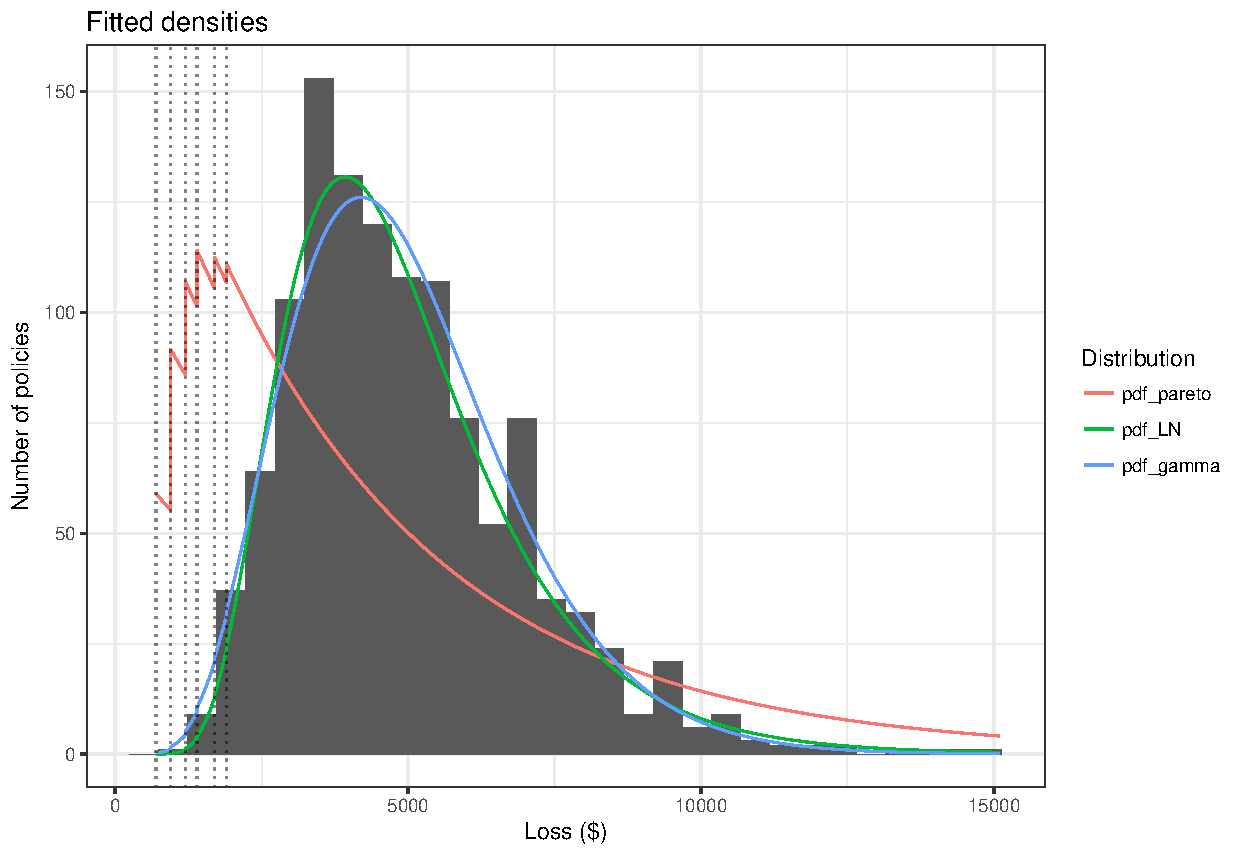
\includegraphics[scale=0.7]{T1_PDF_comparison}
		\caption{Empirical histogram with fitted densities overlay} \label{fig:T1 PDF comparison}
	\end{figure}
	
	In figure \ref{fig:T1 PDF comparison}, we can clearly see that the Pareto distribution's shape is simply not a good fit at all to the observed data. Empirically the data is unimodal with tails on both sides of the peak. The data has a long right tail, also shared by the Pareto distribution. However, the Pareto distribution does not have any tail to the left of its peak, the density simply decreases monotonically. The jumps in theoretical densities is due to the different deductible levels, represented by the dotted vertical lines.\\
	Both the Log Normal and Gamma distribution fit the data much better. To differentiate between the two, it is clearer to look at the CDF.
	
	\begin{figure}[H]
		\centering
		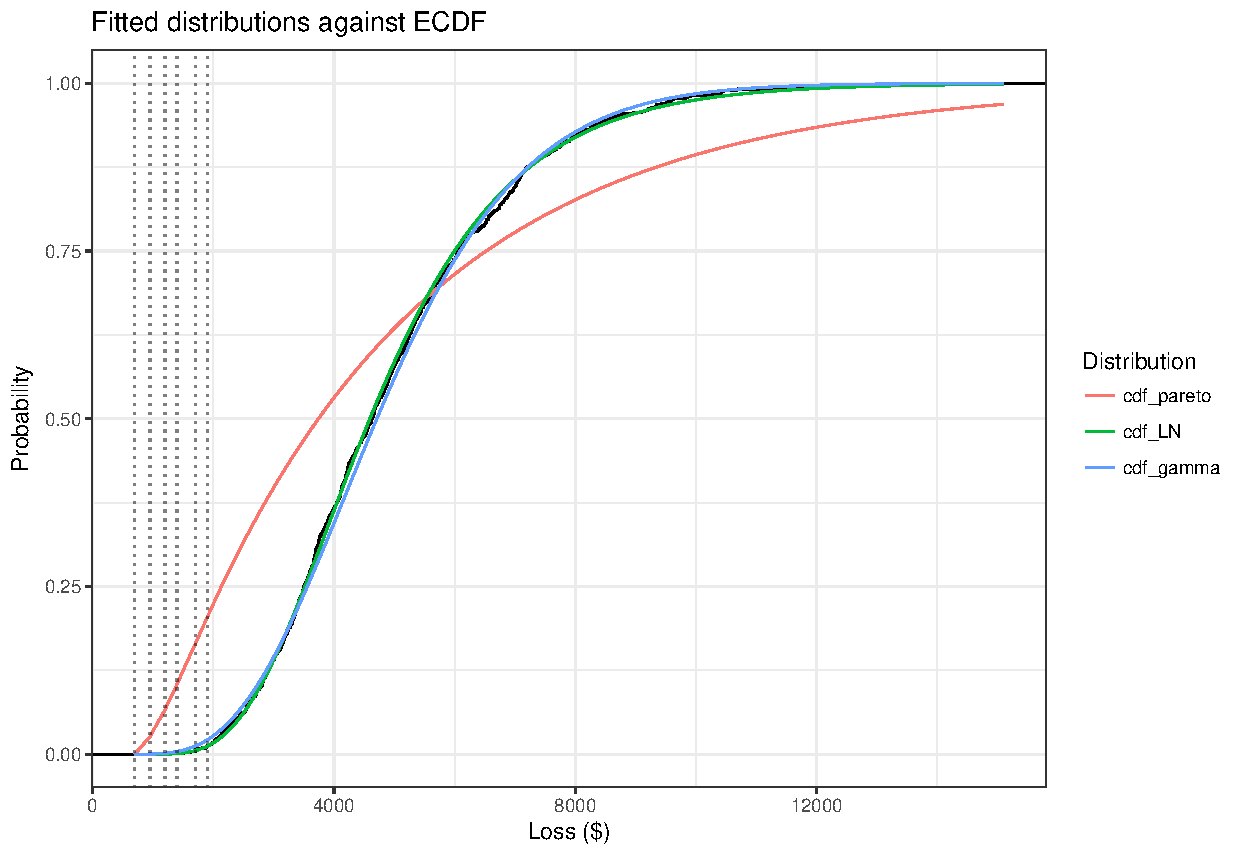
\includegraphics[scale = 0.7]{T1_CDF_comparison}
		\caption{Empirical CDF with fitted distribution overlay} \label{fig:T1 CDF comparison}
	\end{figure} 
	
	In figure \ref{fig:T1 CDF comparison}, it is again clear to see that the Pareto distribution does not fit the data as well as the LN or Gamma. Furthermore, the green line of the LN model follows the black line of the empirical CDF slightly better. This is especially noticeable in the loss range of 4,000 - 7,000, where the Gamma distribution is slightly under the empirical CDF.\\
	\\
	
	\subsubsection{P-P plots}
	The following are P-P plots for the 3 distributions\\
		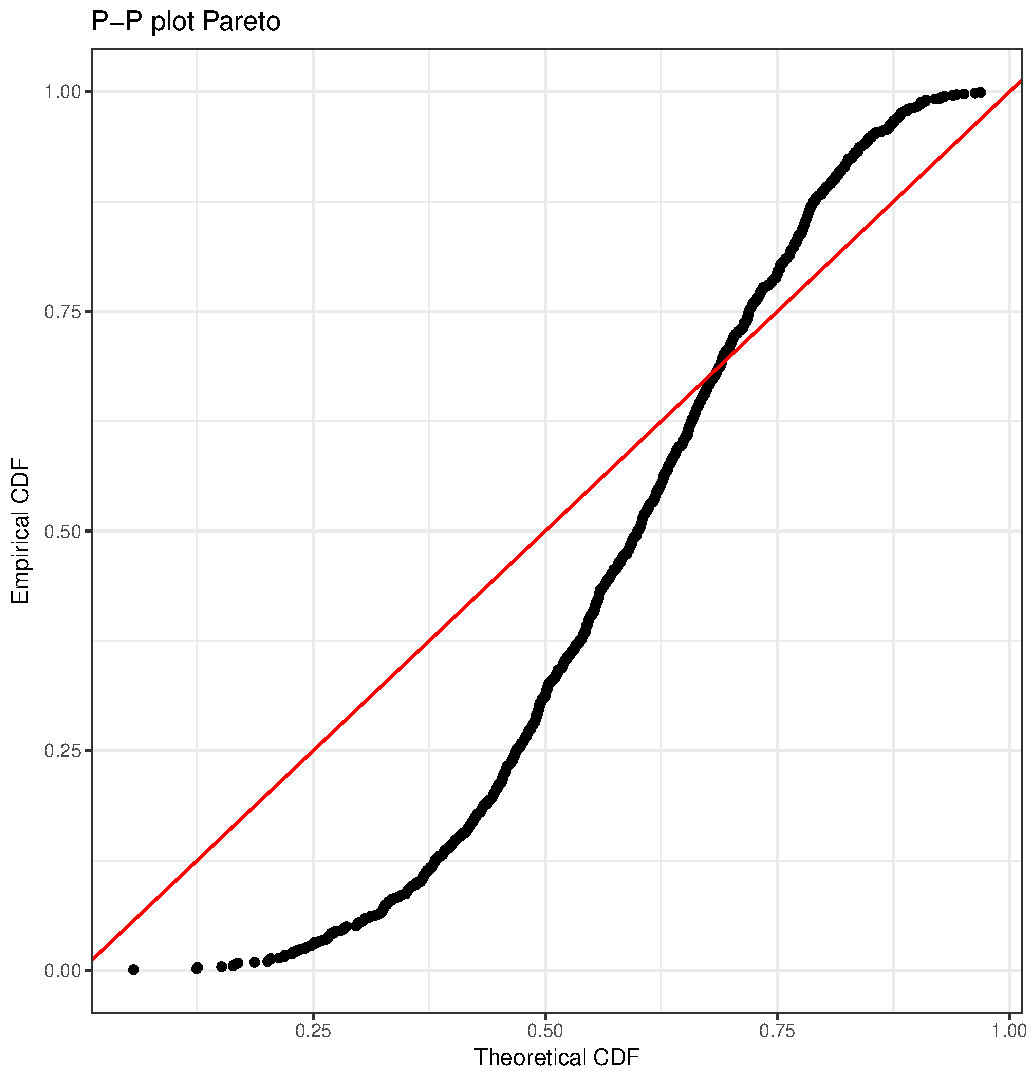
\includegraphics[scale=0.3]{PP_pareto}
		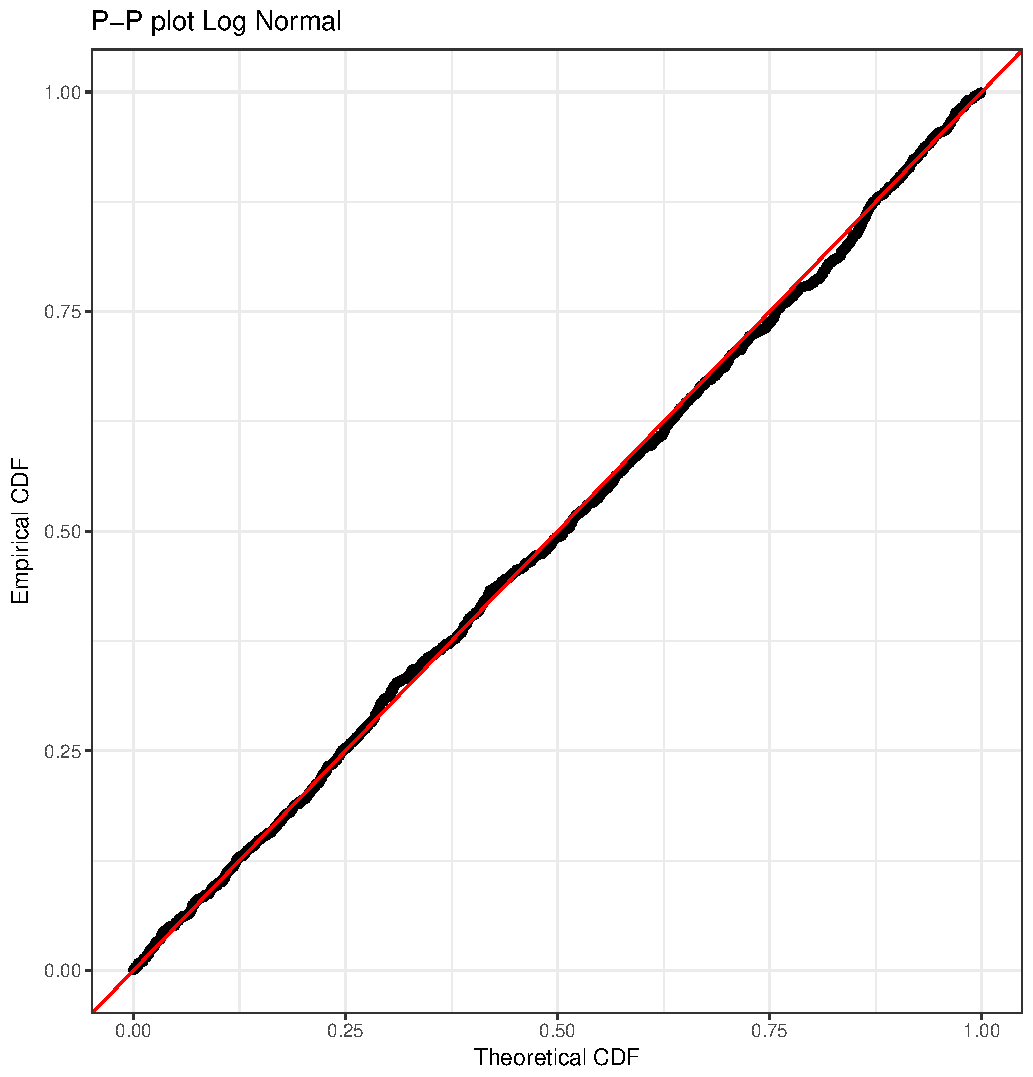
\includegraphics[scale=0.3]{PP_LN}
		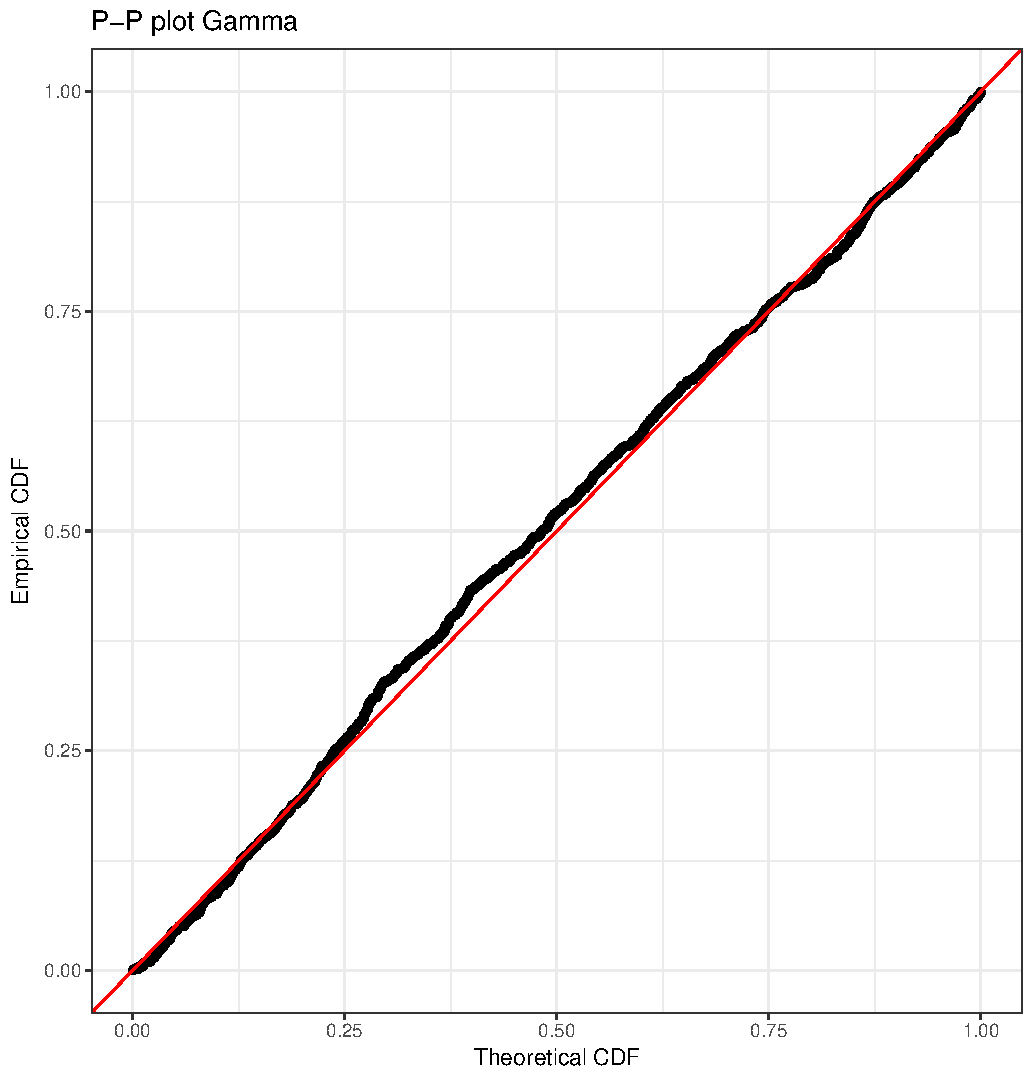
\includegraphics[scale=0.3]{PP_gamma}\\
	It is again clear that the Pareto distribution is not a good fit, with the points not anywhere near close to the $y=x$ line. While both the Log Normal and Gamma distribution seem to be good fits, the Gamma distribution seems to deviate around the middle, again suggesting that the Log Normal model is a better fit.
	
	\subsubsection{Q-Q plots}
	Q-Q plots are better at revealing deviations around the tails. The following are the Q-Q plots for the three distributions.\\
			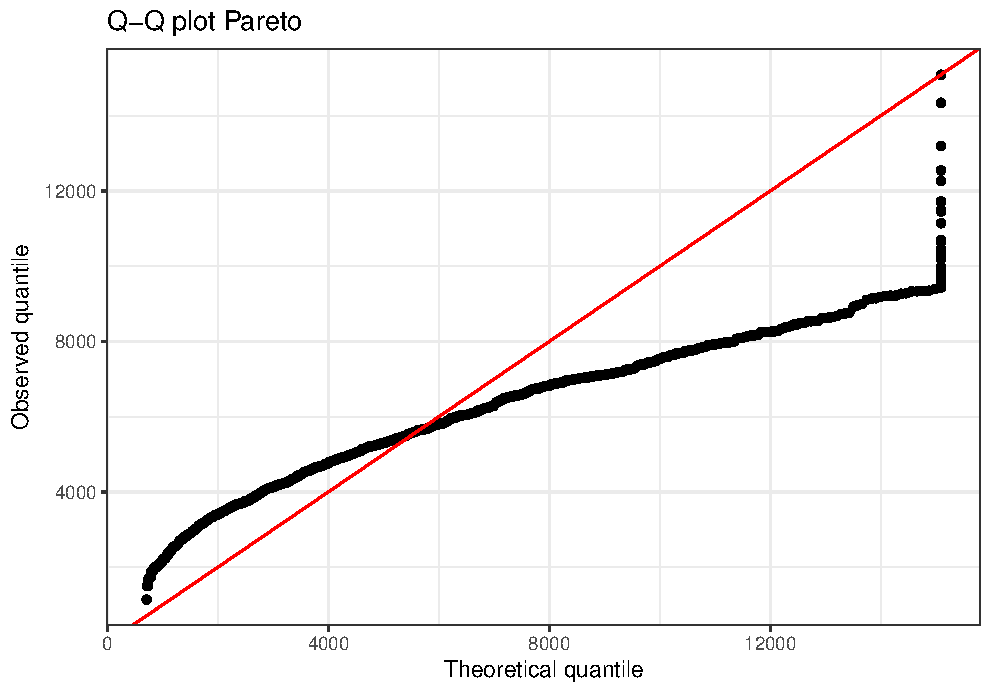
\includegraphics[scale=0.3]{QQ_pareto}
	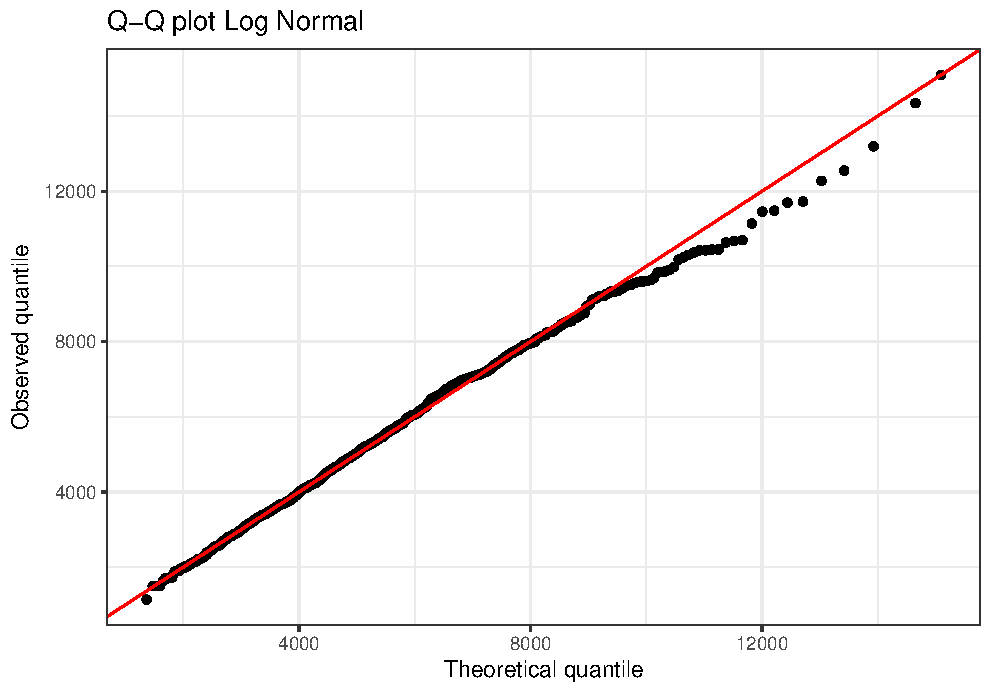
\includegraphics[scale=0.3]{QQ_LN}
	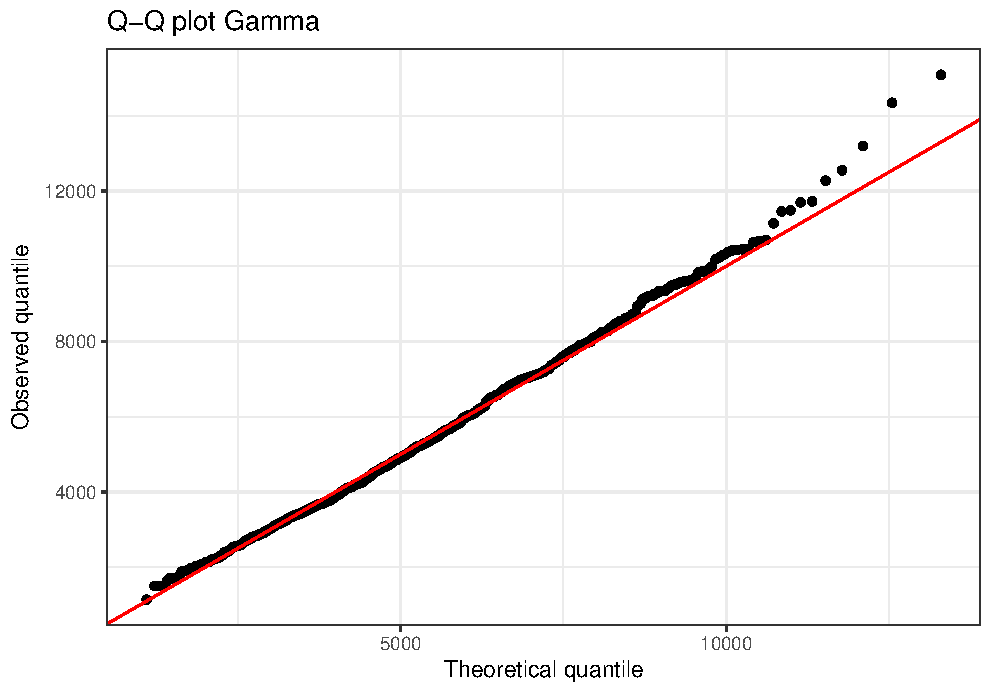
\includegraphics[scale=0.3]{QQ_gamma}\\
	As expected, the Q-Q plot for the Pareto distribution indicates that it is not a good fit anywhere. It is much more interesting to compare the Q-Q plots between the Log Normal and Gamma distribution.\\
	Both are very good fits until the end of the right tail. The Log Normal distribution has a tail that seems too fat for the data given whereas the the Gamma distribution's tail isn't fat enough. That being said, it still appears that the observations appear to follow a Log Normal distribution better as the points move back towards the $y=x$ line for the Log Normal Q-Q plot but less so for the Gamma Q-Q plot.\\
	Furthermore, it can be argued that a model which overestimates loss severity is better than one which underestimates. This is because an overestimation of claims cost lead to higher reserves and decreased probability of ruin. Thus the Log Normal distribution is the most appropriate distribution to model claim size.
	\subsection{Hypothesis tests}
	The Pearson's chi-squared and Kolmogorov-Smirnoff test were conducted for all three distributions. Both these tests reject the null that the data is Pareto distributed and fail to reject the null for the Log Normal and Gamma distribution. This aligns with previous drawn conclusions that the Log Normal and Gamma distributions is a good fit and the Pareto distribution is a bad fit. \\
	Additionally, the p-values of the hypothesis tests are always bigger for the Log Normal distribution, indicating that it has the better fit.
	
	\subsubsection{Pearson's Chi-squared test}
	To conduct this hypothesis test, the data points must be placed in different bins. Table \ref{T1:binned losses} summarises the construction of bins and the number of losses in each one.
	

		
	\begin{table}[H]
		\begin{center}
			\begin{tabular}{ |c|c|} 
			\hline
			Bin range & Number of losses\\ 
			\hline
			$1000 < X \leq 2000$ &  21  \\ 
			$2000 < X \leq 2500$ &  53  \\ 
			$2500 < X \leq 3000$ &  93  \\ 
			$3000 < X \leq 2500$ &  127  \\ 
			$3500 < X \leq 4000$ &  138  \\ 
			$4000 < X \leq 2500$ &  129  \\ 
			$4500 < X \leq 5000$ &  124  \\ 
			$5000 < X \leq 2500$ &  110  \\ 
			$5500 < X \leq 6000$ &  79  \\ 
			$6000 < X \leq 2500$ &  62  \\ 
			$6500 < X \leq 7000$ &  66  \\ 
			$7000 < X \leq 2500$ &  56  \\ 
			$7500 < X \leq 8000$ &  37  \\ 
			$8000 < X \leq 2500$ &  24  \\ 
			$8500 < X \leq 9000$ &  15  \\ 
			$9000 < X \leq 2500$ &  16  \\ 
			$9500 < X \leq 10000$ &  14  \\ 
			$10000 < X \leq 20000$ &  21  \\ 
			
			\hline
			\end{tabular} 
		\end{center}
			\caption{Table of binned losses} \label{T1:binned losses}
	\end{table}

	
	The test statistic is calculated by
	$$\chi^2 = \sum_{i}\frac{(O_i - E_i)^2}{E_i}$$
	Where:
	\begin{align*}
		O_i &= \text{Number of losses in bin $i$}\\
		E_i &= \text{Expected number of losses in bin $i$ given fitted distribution}
	\end{align*}
	Under the null hypothesis (that the data does come from the fitted distribution), the test statistic follows a Chi-squared distribution with degrees of freedom equal to the number of bins minus the number of parameters in the fitted model minus 1:
	$$\sum_{i}\frac{(O_i - E_i)^2}{E_i} \sim \chi^2(n - k - 1)$$
	Where:
	\begin{align*}
		n &= \text{Number of bins} = 18 \\
		k &= \text{Number of parameters in the model} = 2\\
	\end{align*}
	
		
	\begin{table}[H]
		\begin{center}
			\begin{tabular}{ |c|cc|}
				\hline
				Distribution & Test Statistic &      p value       \\ \hline
				Pareto       & 668.54         & $<1\times 10^{-7}$ \\
				Log Normal   & 14.651         &       0.477        \\
				Gamma        & 21.233         &       0.130        \\ 
				\hline
			\end{tabular} 
		\end{center}
		\caption{Results of Chi-squared test} \label{T1:chi-sq results}
	\end{table}

	Table \ref{T1:chi-sq results} show the results of the hypothesis tests. There is significant evidence to show that the data is not Pareto distributed. There is not enough evidence to say that it's not log-normally distributed or Gamma distributed.
	
	\subsubsection{Kolmogorov-Smirnoff test}
	The Kolmogorov-Smirnoff (K-S) test looks at the biggest absolute difference between the empirical CDF and fitted CDF.
	$$KS = \sup_x |F(x) - \hat{F}(x)|$$
	Where:
	\begin{align*}
		F(x) &= \text{The fitted CDF}\\
		\hat{F}(x) &= \text{The empirical CDF}
	\end{align*}
	
	The critical values are given by table \ref{T1: KS critical values}.
	
	\begin{table}[H]
		\begin{center}
		\begin{tabular}{|c|cccccc|}
			\hline
			$ \alpha $ & 20\% & $ 15\% $ & $ 10\% $ & $ 5\% $ & $ 1\% $ & $ 0.1\% $ \\ \midrule
			Formula & $\dfrac{1.073}{\sqrt{n}}$ & $\dfrac{1.138}{\sqrt{n}}$ & $\dfrac{1.224}{\sqrt{n}}$ & $\dfrac{1.358}{\sqrt{n}}$ & $\dfrac{1.628}{\sqrt{n}}$ & $\dfrac{1.94947}{\sqrt{n}}$ \\\midrule
			Value & 0.0312 & 0.0331 & 0.0356 & 0.0394 & 0.0473 & 0.0566 \\\hline
		\end{tabular} \caption{Critical values of the KS test statistic, http://www.real-statistics.com/statistics-tables/kolmogorov-smirnov-table/} \label{T1: KS critical values}
	\end{center}
	\end{table}

	\begin{table}[H]
		\begin{center}
			\begin{tabular}{ |c|cc|}
				\hline
				Distribution & Test Statistic &  p value   \\ \hline
				Pareto       & 0.2647         &  $<0.001$   \\
				Log Normal   & 0.0205         &  $ >0.2 $  \\
				Gamma        & 0.0348         & $ >0.1  $ \\ \hline
			\end{tabular} 
		\end{center}
		\caption{Results of KS test} \label{T1:KS results}
	\end{table}
	
	Table \ref{T1:KS results} shows that, under a significance level of 5\%, the null hypothesis can't be rejected when fitted to the Log Normal or Gamma distribution. Again there is significant evidence suggesting that the data is not Pareto distributed.
	\section{Task 2}
	\subsection{a)}
	Since $S_i \sim $ Gamma$(\alpha,\,\beta)$, we have $\mathbb{E}[S_i] = \frac{\alpha}{\beta}$
	\begin{align*}
		\psi_1(c_0) &= \text{Probability of ruin at time 1}\\
		&= \Pr(C_1<0)\\
		&= \Pr(c_0 + (\pi_1 - S_1)<0)\\
		&= \Pr\left(c_0 + 1.2\frac{\alpha}{\beta}<S_1\right) \qquad \text{since } \pi_i = \pi = 1.2\,\mathbb{E}[S] = 1.2 \frac{\alpha}{\beta}\\
		&= 1-\Pr\left(S_1 \leq c_0 + 1.2 \, \frac{\alpha}{\beta}\right)\\
		&= 1-G\left(c_0+1.2\,\frac{\alpha}{\beta}; \, \alpha, \,\beta\right)
	\end{align*}
	
	
	\subsection{b)}
	This is an expression for the probability that ruin occurs by time 2.
	$$\psi_2(c_0) = \int_{0}^{c_0+\pi}\psi_1(c_0 + \pi - y)\,g(y;\,\alpha,\,\beta)\,dy + 1 - G(c_0 + \pi;\,\alpha,\,\beta)$$
	For the company to be ruined by time 2, one of two disjoint events must occur. Either the company is ruined by time 1, or it survives to time 1 but is ruined by time 2. The above equation is simply the sum of the probabilities of those two events.\\
	The last two terms of the equation represent the probability that ruin will occur by the first time step.\\
	Noting that $\pi = 1.2 \frac{\alpha}{\beta}$ we see that $1 - G(c_0 + \pi;\,\alpha,\,\beta) = \psi_1(c_0)$ as shown in part a). Thus this accounts for the possibility that the insurer is ruined by time step 1.\\\\
	The integral represents the probability that the insurer survives to time step 1, but is ruined by time step 2. Suppose the insurer suffers of a loss of $y$ in time step 1, this leaves them with capital $c_0 + \pi - y$ as the premium, $\pi$, stays constant. For the insurer to have survived, the value of $y$ must be such that $c_0 + \pi - y \geq 0 \Leftrightarrow y \leq c_0 + \pi$.\\
	Assuming that the insurer does survive to time 1, the probability that they are ruined by time 2 is then $\psi_1(c_0 + \pi - y)$. The density of this event occurring, where the insurer suffers a loss of $y$, survives to time 1 but is ruined by time 2, can be expressed as $\psi_1(c_0 + \pi -y)\, g(y;\,\alpha, \,\beta)$ where $g$ is the density of the loss.\\
	The probability can then be found by integrating over all possible values of $y$. Remembering that $y>0$ and $y\leq c_0 + \pi$ , the appropriate integral is then:
	$$\underbrace{\int_{0}^{c_0+\pi}}_\text{all possible values of $y$}\overbrace{\psi_1(c_0 + \pi - y)}^\text{ruin at time 2 given loss of $y$}\,\underbrace{g(y;\,\alpha,\,\beta)}_\text{density of loss equaling $y$}\,dy$$
	Summing these two probabilities together yields
		$$\psi_2(c_0) = \underbrace{\int_{0}^{c_0+\pi}\psi_1(c_0 + \pi - y)\,g(y;\,\alpha,\,\beta)\,dy}_\text{Probability of surviving to time 1 and ruin at 2} + \underbrace{1 - G(c_0 + \pi;\,\alpha,\,\beta)}_\text{Probability of ruin at time 1}$$
	\\
	Assuming $\alpha = 20$ and $\beta = 0.2$, the following was calculated:
		\begin{center}
		\begin{tabular}{ |c|c|} 
			\hline
			$c_0$ & $\psi_2(c_0)$ \\ 
			\hline
			0 &  0.2177  \\ 
			10 & 0.1259 \\ 
			20 & 0.0680 \\ 
			50 & 0.0078\\
			\hline
		\end{tabular}
	\end{center}
	
	\subsection{c)}
	The difficulty in calculating $\psi_t(c_0)$ at higher values of $t$ is the number of calculations involved. These integrals do not have closed form solutions. As a result, numerical methods must be used. For higher values of $t$, it is necessary to take many integrals of integrals, greatly increasing the number of calculations required. Additionally, $g(y;\,\alpha,\,\beta)$ contains $\Gamma(\alpha)$ which must also be calculated using numerical methods.\\
	All this contribute to the rapidly increasing computation complexity of such a calculation and may require many resources.
	
	\subsection{d)}
	\begin{itemize}
		\item \textbf{Give an expression for $\psi_1^*(c_0)$.}\\
		\begin{align*}
			\psi_1^*(c_0)&= \Pr(C^*_1<0)\\
			&= \Pr(c_0 + \pi_1 + S^*_1<0)\\
			&= \Pr(S^*_1 > c_0 + \pi)\\
			&= 1-\Pr(S^*_1 \leq c_0 + \pi)\\
			&= 1 - G^*(c_0 + \pi)
		\end{align*}
		\item \textbf{Provide a recursive expression for $\psi^*_t(c_0)$}\\
		Using a similar logic to part b),
		$$\psi^*_t(c_0) = \psi^*_1(c_0) + \sum_{y = 0}^{\lfloor c_0 + \pi \rfloor}g^*(y)\,\psi_{t-1}^*(c_0 + \pi - y)$$
		Note that the first term represents the probability of immediate ruin. The summation is the probability of ruin by time $t$ given that the company survives time 1. The summation sums over all possible loss values that won't initially ruin the company, from $y=0$ to $c_0-\pi$, the largest integer such that the capital $c_0+\pi-y$ will still be non-negative
		\item \textbf{Comment on the implementation of this expression in comparison to the original case when $S_i$ was continuous.}\\
		The implementation of this algorithm require a much lower number of calculations. This is because of a few reasons. \\
		Firstly, $g^*(y)$ is calculated beforehand and stored. The comparable term in the continuous version must be numerically calculated.\\
		Secondly, each value of $ \psi_{t-1}^*(c_0 + \pi - y) $ can be stored and re-used in later iterations of the algorithm. Conversely, the continuous $\psi$ in the exact algorithm may need to be evaluated from scratch at each iteration.\\
		Lastly, the summation contains $\lfloor c_0 + \pi \rfloor + 1$ terms. Contrastingly, the integral in the continuous recursion must be solved numerically, and so will involve a much larger number of calculations.\\
		The implementation by discretisation of $S$ will drastically reduce the computational effort involved. This comes at a cost of accuracy, but for appropriate discretisation, the discrepancies can be minimal and insignificant.
		
	\end{itemize}

	\subsection{e)}
	\subsubsection{(A)}
	Method of rounding
	\begin{enumerate}[]
		\item $h=1$, $m=150$\\
		\begin{tabular}{ |c|c|} 
			\hline
			$c_0$ & $\psi_2^*(c_0)$ \\ 
			\hline
			0 &  0.2088 \\ 
			10 & 0.1182 \\ 
			20 & 0.0619 \\ 
			50 & 0.0018 \\
			\hline
		\end{tabular}
	
		\item $h=1$, $m=300$\\
		\begin{tabular}{ |c|c|} 
			\hline
			$c_0$ & $\psi_2^*(c_0)$ \\ 
			\hline
			0 &  0.2121 \\ 
			10 & 0.1222 \\ 
			20 & 0.0659 \\ 
			50 & 0.0075 \\
			\hline
		\end{tabular}
	
		\item $h=5$, $m=30$\\
		\begin{tabular}{ |c|c|} 
			\hline
			$c_0$ & $\psi_2^*(c_0)$ \\ 
			\hline
			0 &  0.1876 \\ 
			10 & 0.1045 \\ 
			20 & 0.0539 \\ 
			50 & 0.0014 \\
			\hline
		\end{tabular}

		\item $h=5$, $m=60$\\
			\begin{tabular}{ |c|c|} 
				\hline
				$c_0$ & $\psi_2^*(c_0)$ \\ 
				\hline
				0 &  0.1911 \\ 
				10 & 0.1086 \\ 
				20 & 0.0578 \\ 
				50 & 0.0065 \\
				\hline
			\end{tabular}
	\end{enumerate}

	\subsubsection{(B)}
	Method of upper and lower bounds
	\begin{enumerate}
		\item d = 1
	
			\begin{tabular}{ |c|c|c|} 
				\hline
				$c_0$ & $\psi_2^*(c_0)$ Lower & $ \psi_2^*(c_0) $ Upper \\ 
				\hline
				0 &  0.2190 & 0.2055\\ 
				10 & 0.1269 & 0.1177\\ 
				20 & 0.0688 & 0.0631\\ 
				50 & 0.0080 & 0.0071\\
				\hline
			\end{tabular}
		
		\item d = 5
		
			\begin{tabular}{ |c|c|c|} 
				\hline
				$c_0$ & $\psi_2^*(c_0)$ Lower & $ \psi_2^*(c_0) $ Upper \\ 
				\hline
				0 &  0.2245 & 0.1616\\ 
				10 & 0.1314 & 0.0892\\ 
				20 & 0.0721 & 0.0461\\ 
				50 & 0.0087 & 0.0048\\
				\hline
			\end{tabular}
	\end{enumerate}
	
	\subsubsection{Compare and comment on differences in your results relative to part b).}
	\begin{figure}[H]
		\centering
		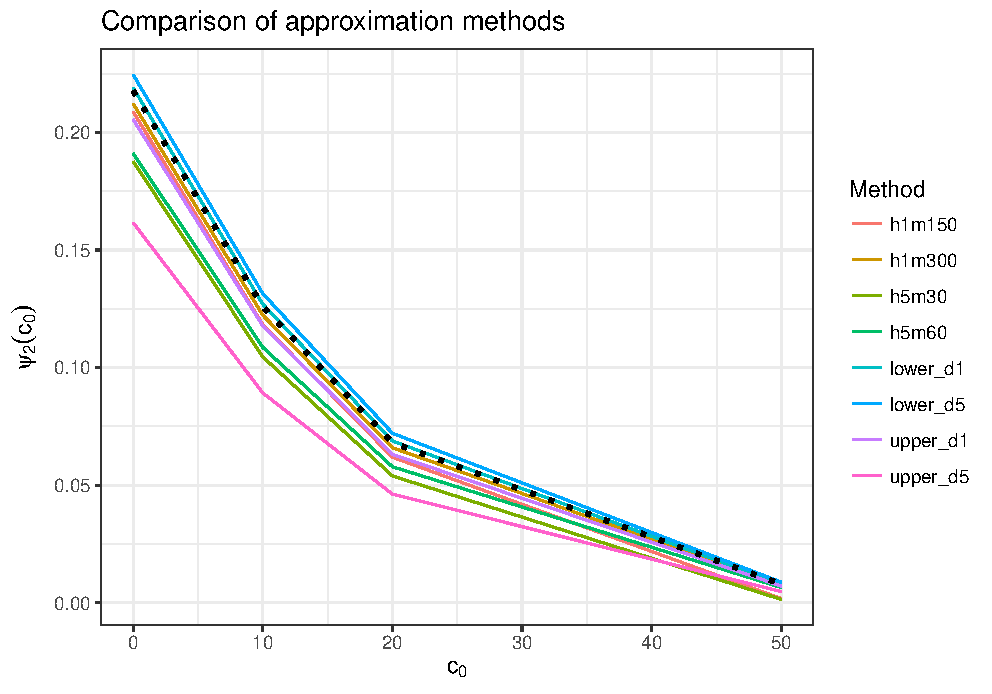
\includegraphics[scale = 1.1]{Approximations.PDF}
		\caption{Comparison of how approximation methods effect the probability of ruin} \label{fig:T2: Approximation comparison}
	\end{figure} 
	The probability of ruin calculated under each approximation method is plotted above along with the true value (dotted black line). There are several key features to note about the different approximation methods.
	\begin{itemize}
		\item Method of rounding
		\begin{itemize}
			\item Smaller values of $h$ yielded a better approximation\\
			This is because the level of granularity is higher with smaller values of h. A higher number of discrete mass points are being used to approximate a continuous distribution.
			\item All the approximated probabilities are lower than the true probability of ruin.
		\end{itemize}
		
		\item Method of upper and lower bounds
		\begin{itemize}
			\item $\psi_2^*(c_0)$ is always smaller than the true probability when using the upper bound approximation and vice versa
			\item The approximation is better with smaller values of $d$. This is because it provides a finer level of detail resulting in more accurate probabilities
		\end{itemize}
	\end{itemize}
	
	\section{Task 3} 
	\subsection{a)}
	\subsubsection{Distribution of $Y_5$}
	Use the method of moment generating functions (mgf) to find the distribution of $Y_5$. Each distribution's mgf is unique to itself, and it can be shown that
	$$Y_5 \sim \text{Gamma}(25, \, 0.8)$$
	Proof:
	\begin{align*}
		M_{Y_{5}}(t) &= \mathbb{E}\left[e^{Y_5\,t}\right]\\
		&=\mathbb{E}\left[e^{t\,\sum_{i = 1}^{5}S_i}\right]\\
		&=\mathbb{E}\left[\prod_{i = 1}^{5}e^{t\,S_i}\right]\\
		&=\prod_{i = 1}^{5}\mathbb{E}\left[e^{t\,S_i}\right] \quad \text{Assuming $S_i$'s are independent of each other}\\
		&= \prod_{i = 1}^{5} M_S(t)\\
		&= \prod_{i = 1}^{5}\left(1 - \frac{t}{\beta}\right)^\alpha\\
		&= \left(1 - \frac{t}{\beta}\right)^{5\alpha}
	\end{align*}	
	Which is the mgf of a Gamma distribution with parameters $5\alpha = 25$, $\beta = 0.8$. Hence $$Y_5 \sim Gamma(25, 0.8)$$
	
	\subsubsection{Distribution function at $x = 10, 20, \ldots, 50$}
	This is calculated numerically through R.
	\begin{center}
		\begin{tabular}{ |c|c|} 
			\hline
			$x$ & $F_{Y_5}(x) $\\ 
			\hline
			10 & 1.172$\times 10 ^{-6}$ \\ 
			20 & 0.0223 \\ 
			30 & 0.4460 \\ 
			40 & 0.9119 \\ 
			50 & 0.9955 \\
			\hline
		\end{tabular}
	\end{center}


	\subsection{b)}
	\subsubsection{Discretise $S_i$ and use Panjer's recursion to approximate $Y_5$}
	Let $F^*_{Y_5}(x)$ denote the CDF calculated using Panjer's recursion and approximated by a discretised $S_i$.
	\begin{center}
		\begin{tabular}{ |c|c|} 
			\hline
			$x$ & $F^*_{Y_5}(x) $\\ 
			\hline
			10 & 1.419$\times 10 ^{-5}$ \\ 
			20 & 0.0324 \\ 
			30 & 0.4837 \\ 
			40 & 0.9226 \\ 
			50 & 0.9961 \\
			\hline
		\end{tabular}
	\end{center}
	\subsubsection{Methodology and assumptions}
	The discretisation of $S_i$ to $ S_i^* $ is done by the method of rounding using parameters $h=1$ and $m = 70$. Let $g_s$ represent the discretised mass function. Then $g_s$ is calculated as
	$$ g_s =
	\begin{cases}
		0 &\text{if $ s $ is not a multiple of $ h $}\\
		0 &\text{if $s<0$} \\
		1 - G(s-\frac{h}{2}) &\text{if $s=hm$}\\
		G(s+\frac{h}{2}) - G(s-\frac{h}{2}) &\text{otherwise}
	\end{cases}
	$$
	Where $G$ is the CDF of $S_i$\\
	$m$ was chosen to be 70 as it was big enough to capture almost all the information of the PDF of $S_i$. This is because $G(70) = \Pr(S_i \leq 70) \approxeq 1$.
	
	To sum five $S_i$ variables, it is assumed that the number of accidents, $N$, follows a binomial distribution with a very high probability parameter.
	$$N \sim Bin(5, 0.997)$$
	A binomial distribution is a member of the (a,b) class of distributions, meaning if $N \sim Bin(n, \,p)$ and $p_r = \Pr(N = r)$, then:
	\[p_r = \left(a + \frac{b}{r}\right)p_{r-1}\]
	Where:
	\begin{flalign*}
		a &=\frac{-p}{1-p}\\
		b&=\frac{(n+1)p}{1-p}
	\end{flalign*}
	
	If $p = 1$. then $N$ would be a constant. However Panjer recursion could not be used as the variables $a,\,b$ would be undefined. $p=0.997$ is a close approximation to a constant, however, with only a 0.015 probability of not evaluating to equal 5. With higher values of $p$, Panjer's recursion is not stable.\\
	\\
	Let $f(s) = \Pr(Y^*_5=5)$ where $Y^*_5 = \sum_{i=1}^{N}S^*$ the sum of the discretised losses with frequency $N \sim Bin(n, \,p)$.\\
	Starting with
	\begin{align*}
		f(0)&=M_N(\ln(g_0))\\
		&=(q+p\times g_0)^n\\
		&=2.688 \times 10^{-13}\\
		&\approx 0
	\end{align*}
	The values of $f(s),\,s = 2,\,3,\ldots$ are recursively calculated using the formula
	\[f(s)=\frac{1}{1-ag_0}\sum_{j=1}^{s}\left(a+b\frac{j}{s}\right) g_jf(s-j)\]
	The distribution function is then simply
	\[F_{Y_5}(s) = \sum_{i=0}^{s}f(i)\]
	\\
	Assumptions:
	\begin{itemize}
		\item Each loss is iid
		\item $N$ is a good enough approximation to 5
		\item The discretisation is a good approximation to the continuous variable
		\item The loss can take the value of 0. \\Although this does not reflect the original distribution, the discretised mass at 0 is insignificantly small with $g_0<0.0001$. \\
		Despite a simple correction that could have been made, it would not have had a material difference. Additionally, $f(0)$ would had to have been non-zero anyways as $\Pr(N=0)>0$.
	\end{itemize}
	
	\subsection{Comparison}
	
	Table \ref{Table:T3 value comparison} compares the approximation to the true distribution side by side. The approximation always overestimates the true distribution value. However it is a small overestimate, with the largest only being a couple percent higher than true value.\\
	\begin{table}[H]
		\begin{center}
			\begin{tabular}{ |c|ccc|} 
				\hline
				$x$ & $F^*_{Y_5}(x) $& $F_{Y_5}(x) $ & Difference \\ 
				\hline
				10 & 1.419$\times 10 ^{-5}$ & 1.172$\times 10 ^{-6}$ & $1.3 \times 10^{-5}$\\ 
				20 & 0.0324 & 0.0223 & 0.0101\\ 
				30 & 0.4837 & 0.4460 & 0.0377\\ 
				40 & 0.9226 & 0.9119 & 0.0107\\ 
				50 & 0.9961 & 0.9955 & 0.0006\\
				\hline
			\end{tabular} \caption{Comparison of approximation and true value} \label{Table:T3 value comparison}
		\end{center}
	\end{table}
	
	\begin{figure}[H]
		\centering
		\includegraphics[scale = 0.6]{panjer_combined.PDF}
		\caption{Comparison of approximation using Panjer recursion and discretisation to true probabilities} \label{fig:T3 combined graph}
	\end{figure} 
	Figure \ref{fig:T3 combined graph} shows the approximated mass and distribution functions in grey and the true density and distribution in red. Visually, the approximation seems to follows the true values very closely.
	
	
	
	
	
	\appendix
	\section{Task 1}
	\subsection{MLE for Pareto}
	The Pareto distribution with shape parameter $ \alpha $, scale parameter $ \lambda $ have the following distributions:
	\begin{align*}
	f(x) &= \frac{\alpha \lambda^\alpha}{(\lambda+x)^{\alpha + 1}}, \quad x > 0\\
	F(x) &= 1-\left(\frac{\lambda}{\lambda + x}\right)^\alpha, \quad x > 0
	\end{align*}
	From equation (\ref{loglik}) we know that 
	\begin{align*}
		l&=\sum_{i=1}^{n}\left[\ln(f(x_i)) - \ln(1-F(d_i))\right]\\
		&=\sum_{i=1}^{n}\left[\ln\left(\frac{\alpha\lambda^\alpha}{(\lambda + x_i)^{\alpha+1}}\right) - \ln\left(\left(\frac{\lambda}{\lambda + d_i}\right)^\alpha\right)\right]\\
		&=\sum_{i=1}^{n}\left[\ln(\alpha) - (\alpha + 1)\ln(\lambda + x_i) + \alpha\ln(\lambda+d_i)\right]\\
	\end{align*}
	Differentiating with respect to $\alpha$ and $\lambda$ yields:
	\begin{align}
		\frac{\partial l}{\partial\alpha}&=\frac{n}{\alpha} +\sum_{i=1}^{n}\ln\left(\frac{\lambda + d_i}{\lambda+x_i}\right)\\
		\frac{\partial l}{\partial\lambda}&=\sum_{i=1}^{n}\left[\frac{-(\alpha+1)}{\lambda+x_i}+\frac{\alpha}{\lambda+d_i}\right]
	\end{align}

	We set the first derivatives to $0$ and solve to to find the MLE:
	\begin{align}
		\frac{\partial l}{\partial\alpha}&=0 \nonumber\\
		\Leftrightarrow 0 &= \frac{n}{\hat{\alpha}} +\sum_{i=1}^{n}\ln\left(\frac{\hat{\lambda} + d_i}{\hat{\lambda}+x_i}\right) \nonumber\\
		\Leftrightarrow \hat{\alpha} &= \frac{-n}{\sum_{i=1}^{n}\ln\left(\frac{\hat{\lambda} + d_i}{\hat{\lambda}+x_i}\right)}\\
	\end{align}

	\section{R code}
	\subsection{Data pre processing}
	\lstinputlisting{"C:/Users/johnn/Dropbox/Uni/2017 S2/ACTL3162/Assignment/Codes/Support code/importing.R"}
	\subsection{Task 1}
	\lstinputlisting{"C:/Users/johnn/Dropbox/Uni/2017 S2/ACTL3162/Assignment/Codes/Task1.R"}
	\subsection{Task 2}
	\lstinputlisting{"C:/Users/johnn/Dropbox/Uni/2017 S2/ACTL3162/Assignment/Codes/Task2.R"}
	\subsection{Task 3}
	\lstinputlisting{"C:/Users/johnn/Dropbox/Uni/2017 S2/ACTL3162/Assignment/Codes/Task3.R"}
\end{document}